\section{Appendix A: Relational Algebra for Rule Evaluation}
Consider the following example:
\begin{align*}
&Order(1, 2),\; Order(2, 3). \quad\quad\quad\quad\quad\quad\quad\quad\quad[r_1]\\
&Order(x, z) \coloneqtwo Order(x, y),\; Order(y, z). \;\quad\quad\quad[r_2]
\end{align*}
\noindent
Rule $[r_1]$ states that the orders $1, 2$ and $2, 3$ holds. Rule $[r_2]$ states that the binary $Order$ relation is transitive. The BUN evaluation proceeds as follows. For each rule that is evaluated, an artificial body-relation $B$ is introduced. The body-relation will be incrementally populated and extended through the evaluation of the atoms in the body. 

Initially, the relation associated with each atom is unnamed, i.e. the columns of the relation have no name-restrictions. Given a rule $r$, we order the atoms from the body of the rule as $A_1, \ldots, A_n$. We will consider each atom in turn and use the body relation $B$ as an accumulator. The equations describing the rule-evaluation process is as follows (the notation is explained below):
\begin{align*}
B^{0} &\leftarrow \top \\
B^{i + 1} &\leftarrow B^{i} \bowtie \sigmatwo_{Term(A_{i + 1})}\;(A_{i + 1}), \; i = 0, \ldots, n - 1\\
H & \leftarrow H \cup \Pi_{Term(H)}(B^n)
\end{align*}
\noindent
The body relation is initially assigned to $\top$ denoting an unknown relation: $\top \bowtie R = R \bowtie \top = R$. The $Term$ function gives the terms in the given atom. $H$ is the head of rule $r$. A selection is then done for the atom. The special selection operator is denoted $\sigmatwo$. Informally it selects a set of tuples from the relation associated with the atom that satisfies the constraints imposed by the terms of the atom. As a more formal example:
\begin{align*}
\sigmatwo_{x,x,y,c} = \rho_{x/x_1, y/y_1} \circ \Pi_{x_1, y_1} \circ \sigma_{x_1 = x_2, C_1 = c} \circ \rho_{x_1/N_0, x_2/N_1, y_1/N_2, C_1/N_3}
\end{align*}

The selection is for three variables $x, x, y$ and a constant $c$. First the rename operator $\rho$ is used to rename the columns of the relation ($N_i$ is an artificial initial name for column $i$). Then the ordinary $\sigma$ operator selects all tuples such that the corresponding variables and constants match under the given naming. The result of the selection is then projected (discarding duplicates and constants) using the projection operator $\Pi$, and finally the inverse renaming is performed.

The selection result is joined ($\bowtie$) with the current body relation $B^{i}$ to form the next body relation $B^{i + 1}$. In our example (assuming that $r_1$ has been evaluated) we get:
\begin{align*}
B^{1} &\leftarrow \sigmatwo_{x, y}\;(Order) = \{(1, 2), (2, 3)\}_{x, y}\\
B^{2} &\leftarrow B^{1} \bowtie (\sigmatwo_{y, z}\;(Order) = \{(1, 2), (2, 3)\}_{y, z})\\
      &= \{(1, 2), (2, 3)\}_{x, y} \bowtie \{(1, 2), (2, 3)\}_{y, z}\\
      &= \{(1,2,3)\}_{x,y,z}
\end{align*}
\noindent
Finally we project the result of $B^n$ and add the new tuples to the head relation:
\begin{align*}
Order & \leftarrow Order \cup (\Pi_{x,z}(\{(1,2,3)\}_{x,y,z}) = \{(1,3)\})
\end{align*}
\noindent
The process is iterated until a fix-point is found, i.e. until no new tuples can be derived from the set of rules. In our example, iterating $[r_2]$ again gives no new tuples and so the $Order$ relation has been computed as: $\{(1,2), (1,3), (2,3) \}$.
\clearpage
\section{Appendix B: Correctness of Type Algorithm}
For an atom $A$ in the type algorithm, let the corresponding set of tuples be denoted $A_R$. The typing algorithm reports a type error in one of two cases:
\begin{align*}
&\exists A \in PRED_{P_T}.\;\;|A_R| > 1 \quad\quad (1)\\
&\exists A \in PRED_{P_T}.\;\;|A_R| = 0 \quad\quad (2)
\end{align*}
\noindent
A Datalog program $P$ is said to be \textit{well-typed} if:
\begin{align*}
\forall A \in PRED_{P_T}. \;\; |A_R| = 1 \quad\quad (3)
\end{align*}
\noindent
Let $Pos(x, A)$ give the coordinate of term $x$ in predicate $A$, and $A[n]$ give type of $A$ at coordinate $n$. A rule with two atoms using the same variable name gives a \textit{type constraint}:
\begin{align*}
\infer[(\textit{C-VarLeft})]{A[Pos(x, A)] = \tau}{\begin{array}{c c} &B[Pos(x, B)] = \tau\\&\exists Rule: \ldots, A( \ldots, x, \ldots), \ldots, B(\ldots, x, \ldots), \ldots\end{array}}
\end{align*}
\begin{align*}
\infer[(\textit{C-VarRight})]{B[Pos(x, B)] = \tau}{\begin{array}{c c} &A[Pos(x, A)] = \tau\\&\exists Rule: \ldots, A( \ldots, x, \ldots), \ldots, B(\ldots, x, \ldots), \ldots\end{array}}
\end{align*}
\noindent
Let the type of a constant term $t$ be given by $T(t)$. We get the following constraint for constants:
\begin{align*}
\infer[(\textit{C-Constant})]{A[Pos(t, A)] = T(t)}{\exists Clause\;C: \ldots A(\ldots, t, \ldots), \ldots, \;\; t : Constant } 
\end{align*}
\noindent
Finally, the semantics of $TYPEOF$ is added as a rule:
\begin{align*}
\infer[(\textit{C-TypeOf})]{A[Pos(\tau, TYPEOF)] = \tau}{\exists Fact: \; TYPEOF('A,\ldots, \tau, \ldots) } 
\end{align*}

\noindent
We say that a type algorithm is \textit{correct} if the type solution satisfies the listed constraints together with the additional requirement that in a valid type assignment, each predicate is assigned exactly one type (property (3) above). \textit{C-TypeOf} is satisfied by the type-checking algorithm by construction. We now show that it additionally satisfies \textit{C-Constant} and \textit{C-Var}. Together with properties (1), (2) this is enough to show correctness since $(3) \iff \neg ((1) \lor (2))$.

\paragraph{Proposition: } \textit{The type-checking algorithm satisfies C-Constant}\NL
A clause is either a fact or a rule. All facts are lifted to the type level and thus trivially satisfy \textit{C-Constant}. Thus assume that have a rule with a constant use in an atom A. We will get a corresponding type-rule with head $R_i$ with $A$ unconditionally in the body:
\begin{align*}
R_i(\ldots) \coloneqtwo \ldots A(\ldots, c, \ldots) \ldots
\end{align*}
By the Datalog semantics, $|R_i| > 0$ if can derive that A contains a fact with the constant (lifted type) $c$ at coordinate $Pos(c, A)$. Since there is no other clause that derives facts for $R_i$, this is the only way to satisfy $|R_i| = 1$ (if $|R_i| \neq 1$ then algorithm fails due to (1), (2)).\\\hspace*{200pt}$\blacksquare$

\paragraph{Proposition: } \textit{The type-checking algorithm satisfies C-Var*}\NL
Since C-VarLeft and C-VarRight are completely symmetrical it suffices to show for C-VarLeft.
Assume that we have a rule $R$ that gets transformed to a type-rule with head $R_i$:
\begin{align*}
&R_i(\ldots, x, \ldots) \coloneqtwo \ldots, A( \ldots, x, \ldots), \ldots, B(\ldots, x, \ldots), \ldots\\
&B[Pos(x, B)] = \tau
\end{align*}
\noindent
The algorithm reports a type error iff (3) does not hold for the type-program. Thus $B[Pos(x, B)]$ has $\tau$ as the only member.
By the Datalog semantics (and from the fact that no other rule populates $R_i$), (3) holds if and only if $A[Pos(x, A)] = \tau$. \\\hspace*{200pt}$\blacksquare$
\clearpage
%\section{Appendix C: Plots for Experimental Data}
%\begin{figure}[!htb]
%%	\hspace*{-25pt}
%%	\begin{minipage}[b]{.5\textwidth}
%		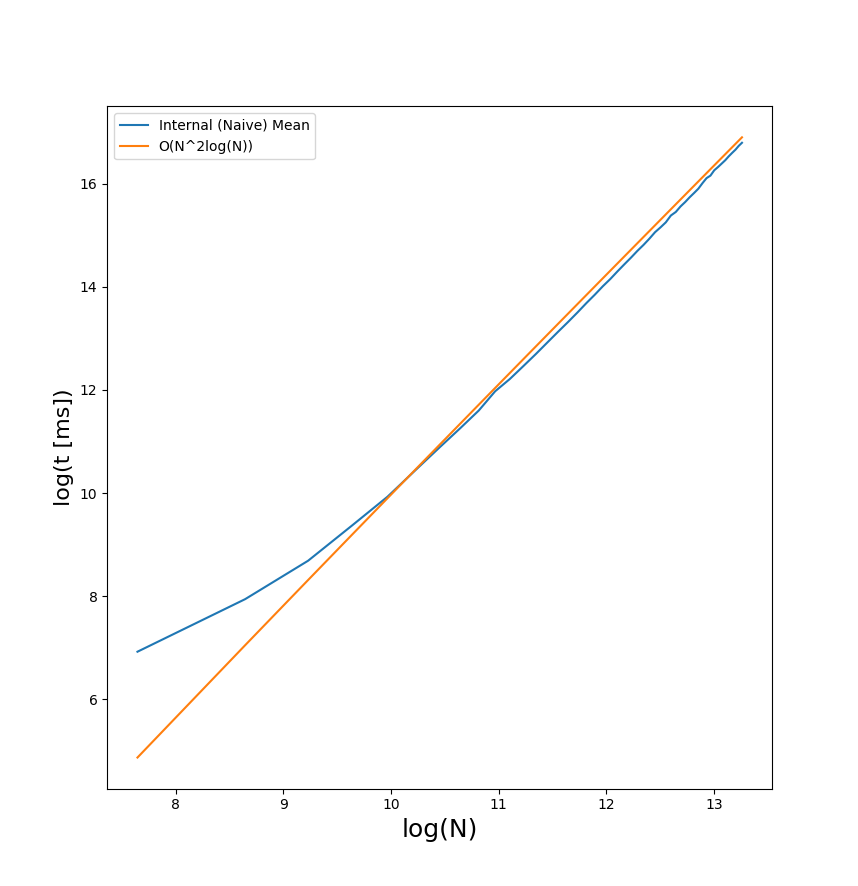
\includegraphics[width=0.9\linewidth]{img/internalloglog.png}
%	%\end{minipage}%
%%	\hspace*{-40pt}
%%	\begin{minipage}[b]{.5\textwidth}
%%		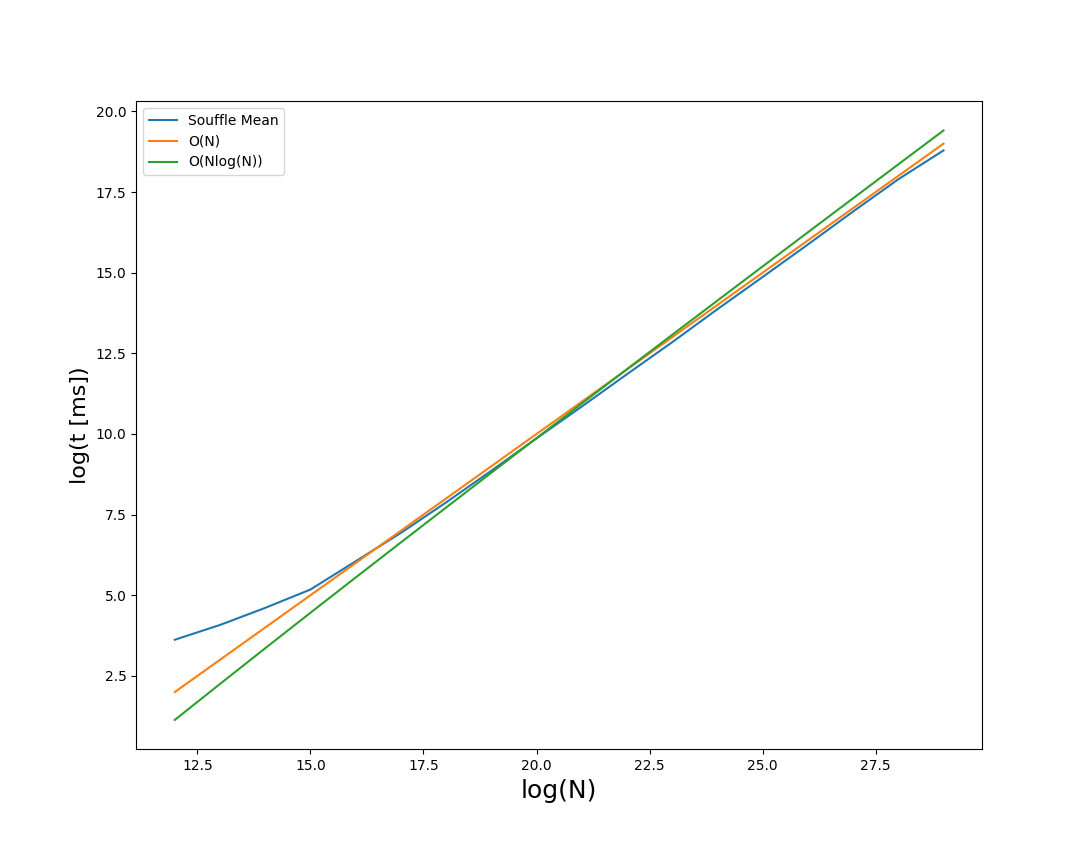
\includegraphics[scale=0.35]{img/souffleloglog.png}
%%	\end{minipage}
%%	\label{figure:natExperimental}
%	\caption{Nat Example, Internal Evaluation (Naive)}
%\end{figure}
%\begin{figure}[!htb]
%	\centering
%	%	\hspace*{-25pt}
%	%	\begin{minipage}[b]{.5\textwidth}
%	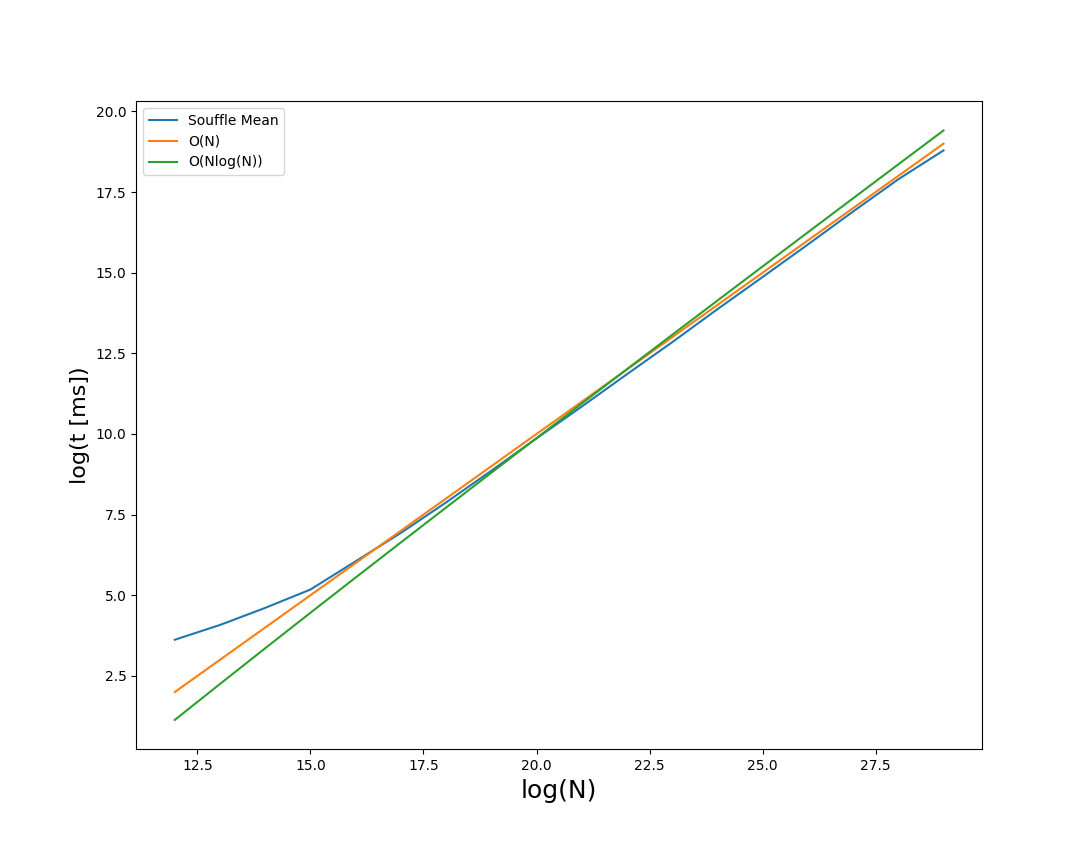
\includegraphics[width=1.0\linewidth]{img/souffleloglog.png}
%	%\end{minipage}%
%	%	\hspace*{-40pt}
%	%	\begin{minipage}[b]{.5\textwidth}
%	%		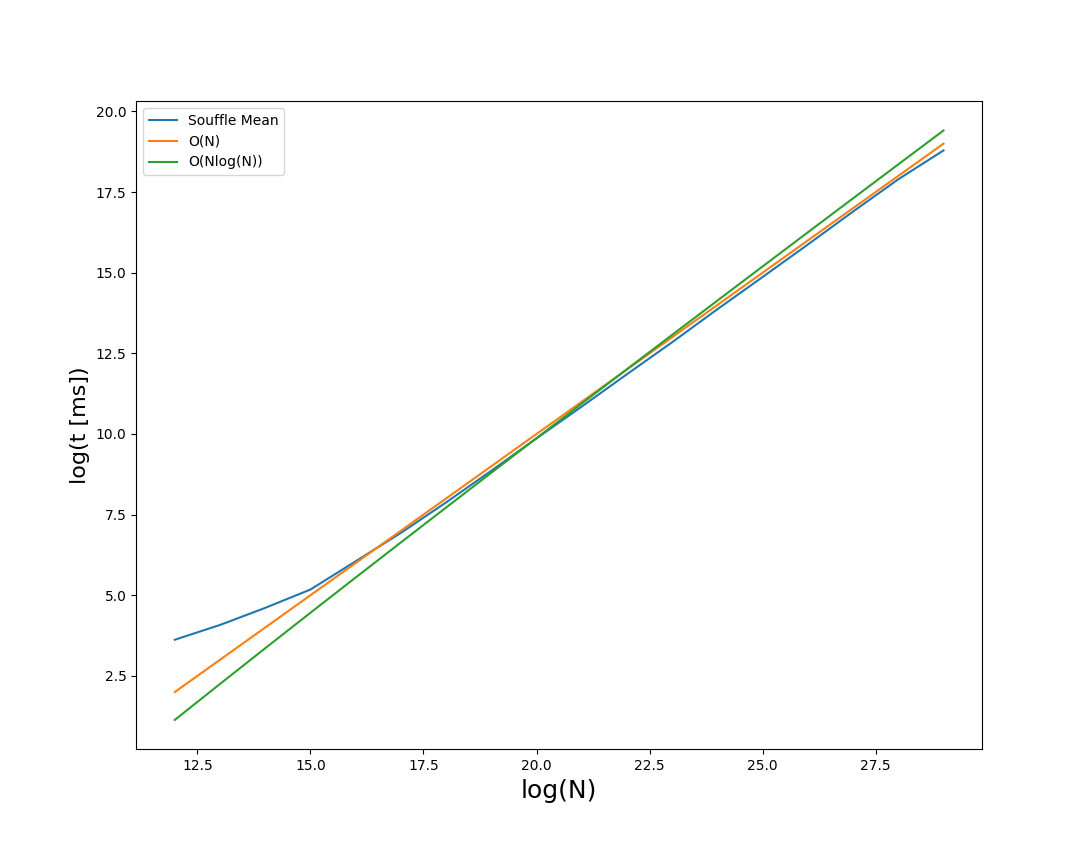
\includegraphics[scale=0.35]{img/souffleloglog.png}
%	%	\end{minipage}
%	%	\label{figure:natExperimental}
%	\caption{Nat Example, Souffle Evaluation (Semi-Naive)}
%\end{figure}
%\begin{figure}[!htb]
%	\centering
%	%	\hspace*{-25pt}
%	%	\begin{minipage}[b]{.5\textwidth}
%	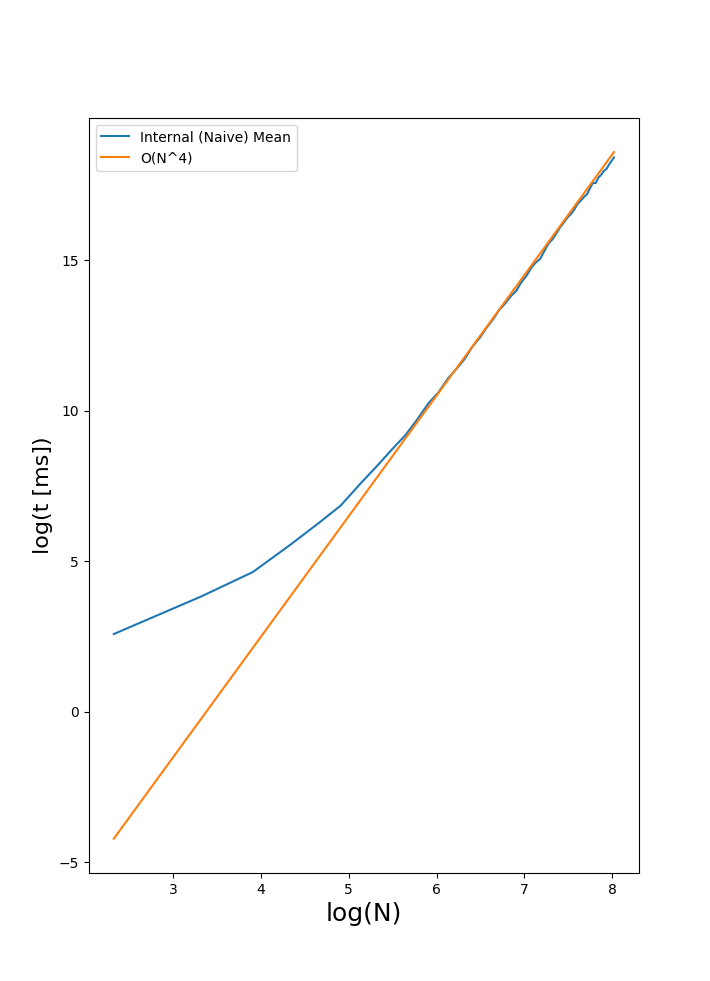
\includegraphics[width=1.0\linewidth]{img/ancestorInternal.png}
%	%\end{minipage}%
%	%	\hspace*{-40pt}
%	%	\begin{minipage}[b]{.5\textwidth}
%	%		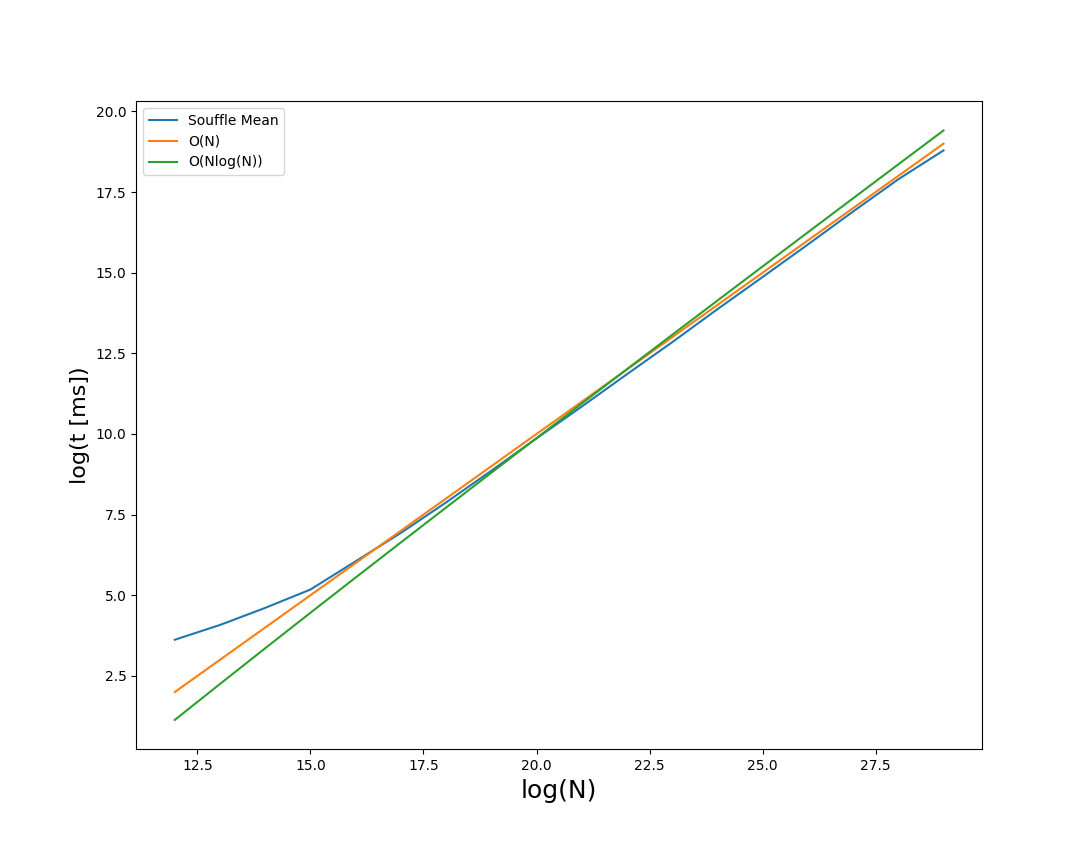
\includegraphics[scale=0.35]{img/souffleloglog.png}
%	%	\end{minipage}
%	%	\label{figure:natExperimental}
%	\caption{Nat Example, Souffle Evaluation (Semi-Naive)}
%\end{figure}
%\begin{figure}[!htb]
%	\centering
%	%	\hspace*{-25pt}
%	%	\begin{minipage}[b]{.5\textwidth}
%	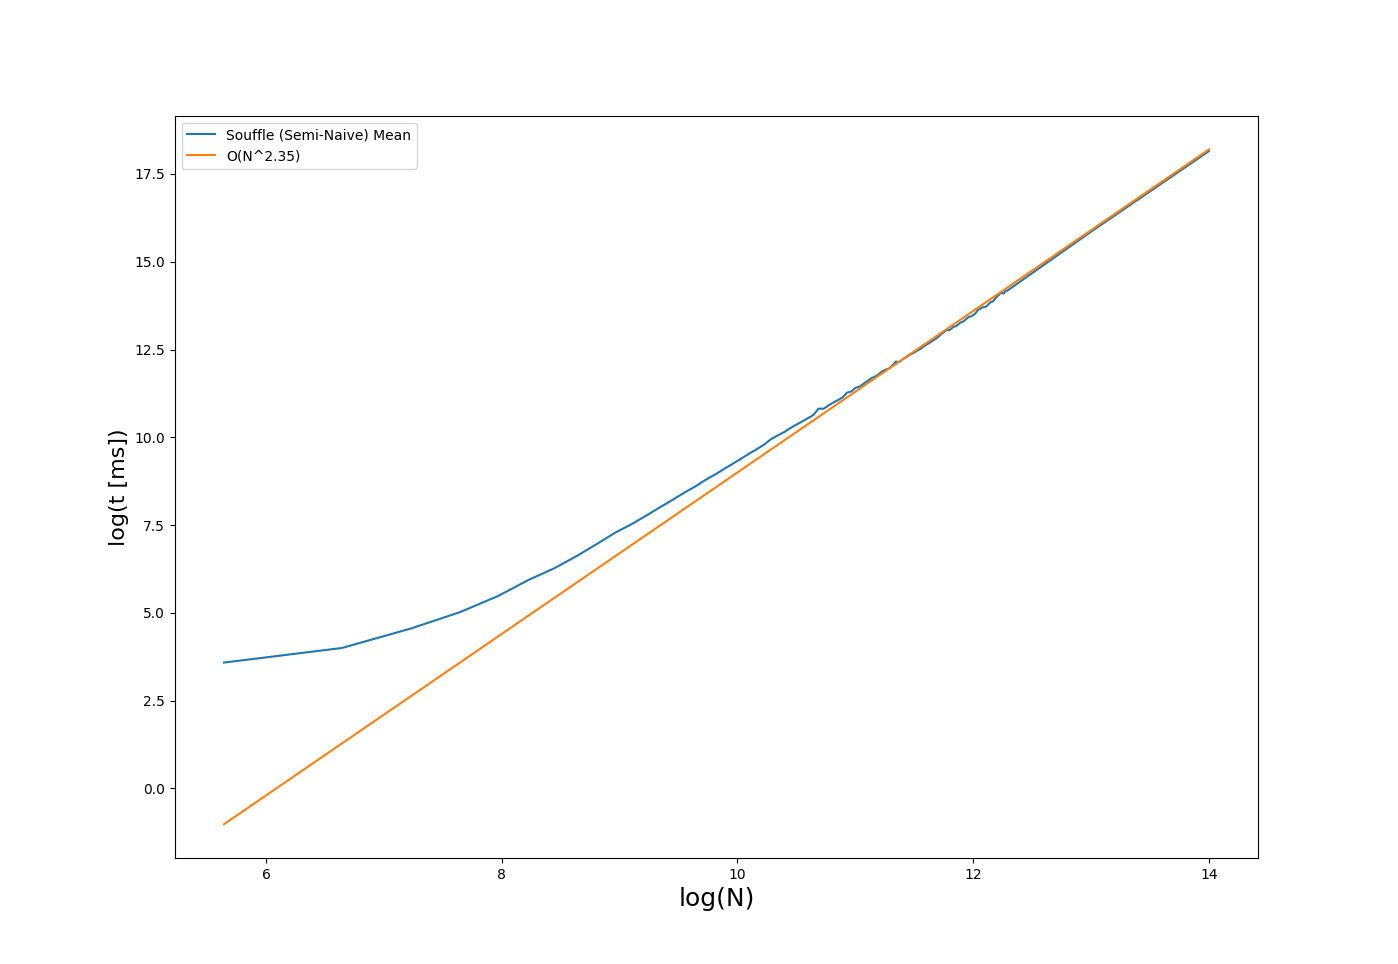
\includegraphics[width=1.0\linewidth]{img/ancestorSouffle.png}
%	%\end{minipage}%
%	%	\hspace*{-40pt}
%	%	\begin{minipage}[b]{.5\textwidth}
%	%		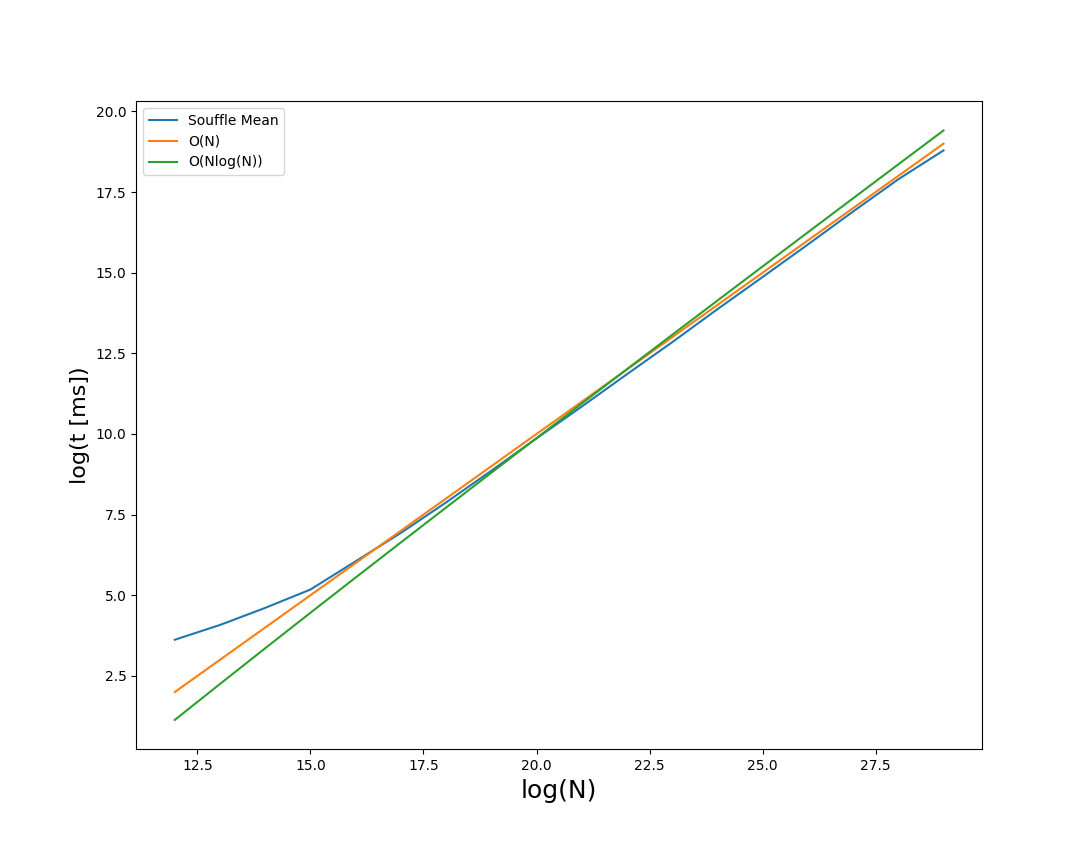
\includegraphics[scale=0.35]{img/souffleloglog.png}
%	%	\end{minipage}
%	%	\label{figure:natExperimental}
%	\caption{Nat Example, Souffle Evaluation (Semi-Naive)}
%\end{figure}
%
%
%%\begin{figure*}[!t]
%%	\hspace*{-70pt}
%%	\begin{minipage}[b]{.5\textwidth}
%%		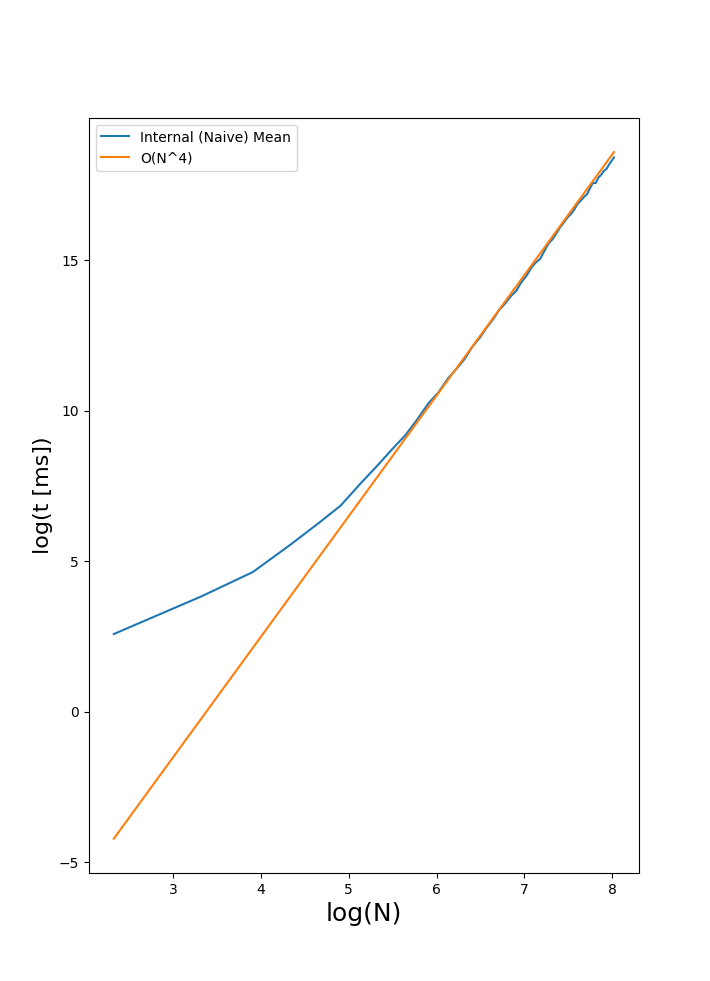
\includegraphics[scale=0.345]{img/ancestorInternal.png}
%%	\end{minipage}%
%%	\hspace*{-70pt}
%%	\begin{minipage}[b]{.5\textwidth}
%%		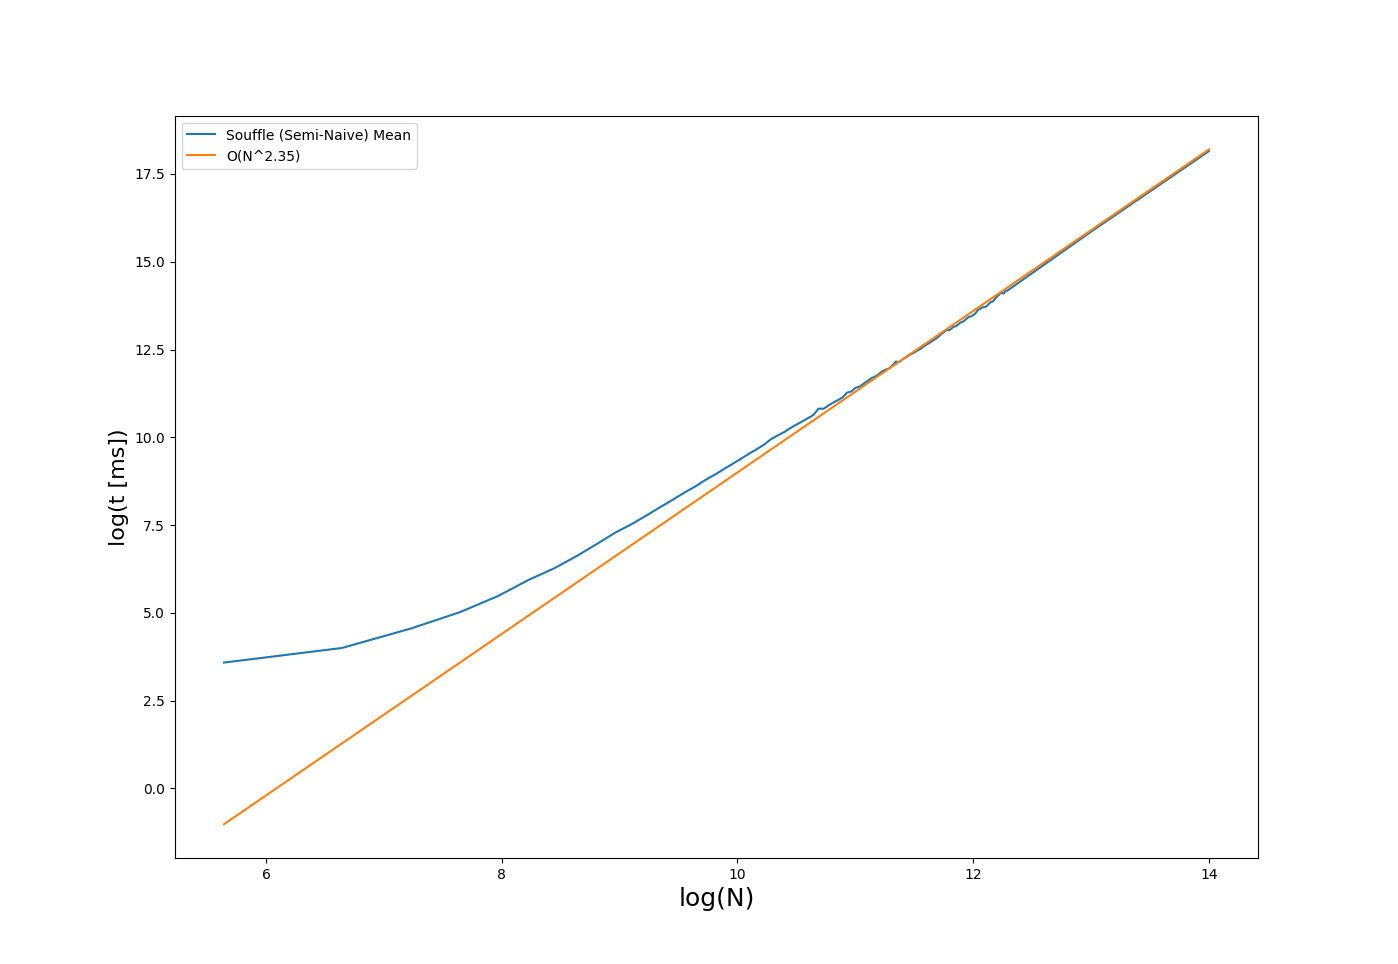
\includegraphics[scale=0.35]{img/ancestorSouffle.png}
%%	\end{minipage}
%%	\label{figure:ancestorExperimental}
%%	\caption{Ancestor Example, \textbf{Left: } Internal (Naive), \textbf{Right: } Souffle (Optimized Semi-Naive)}
%%\end{figure*}